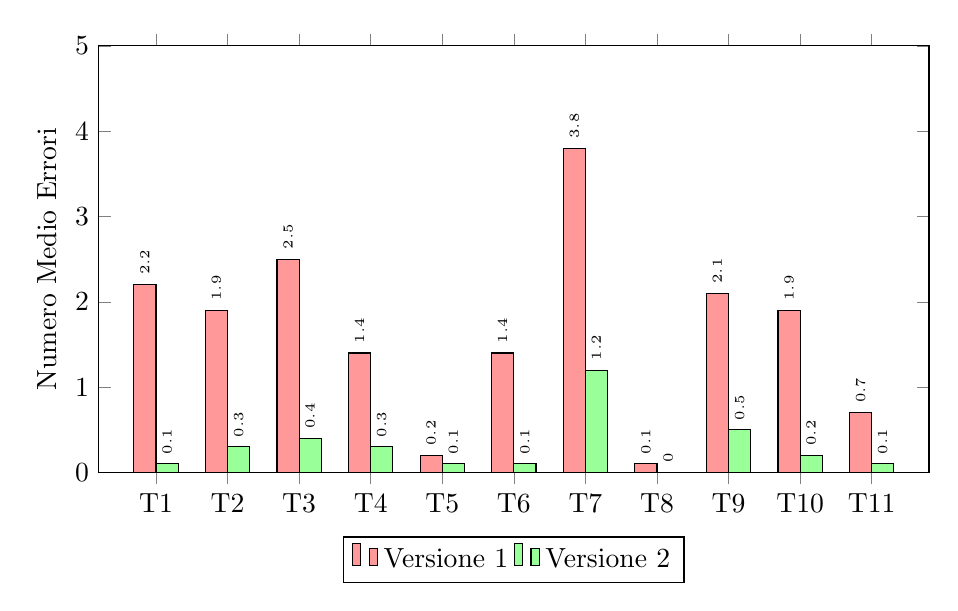
\begin{tikzpicture}
    \begin{axis}[
        ybar=0pt,
        bar width=8pt,
        enlarge x limits=0.08,
        legend style={at={(0.5,-0.15)}, anchor=north, legend columns=-1},
        ylabel={Numero Medio Errori},
        symbolic x coords={T1, T2, T3, T4, T5, T6, T7, T8, T9, T10, T11},
        xtick=data,
        nodes near coords,
        nodes near coords align={vertical},
        every node near coord/.append style={font=\tiny, rotate=90, anchor=west},
        width=\textwidth,
        height=7cm,
        ymin=0,
        ymax=5
    ]
        \addplot[fill=red!40] coordinates { (T1,2.2) (T2,1.9) (T3,2.5) (T4,1.4) (T5,0.2) (T6,1.4) (T7,3.8) (T8,0.1) (T9,2.1) (T10,1.9) (T11,0.7) };
        \addplot[fill=green!40] coordinates { (T1,0.1) (T2,0.3) (T3,0.4) (T4,0.3) (T5,0.1) (T6,0.1) (T7,1.2) (T8,0) (T9,0.5) (T10,0.2) (T11,0.1) };
        \legend{Versione 1, Versione 2}
    \end{axis}
\end{tikzpicture}